\startchapter{Results}
In order to provide a more comprehensive prediction of the sensitivity of the analysis regions to the signal model we perform an exclusion fit. In an exclusion fit, the signal model plus the standard model background is taken as the null hypothesis and is tested against the alternative hyposthesis of the background only model. The following chapter describes the process of the fit and demonstrates the results.

\section{Statistical Framework}
\label{section:stats}
In each signal region we create a histogram of events consisting of several bins in a chosen variable. The expectation value for the number of events in a single bin is:
\begin{equation}
E[n_i] = \mu s_i(\boldsymbol{\theta}) + b_i(\boldsymbol{\theta})
\end{equation}
where $\mu$ is the parameter of interest, the signal strength, which is 0 in the background-only case and 1 in the nominal signal model. $\boldsymbol{\theta}$ is the set of nuisance parameters, and $s_i$ and $b_i$ are the expected number of signal and background events in bin $i$:
\begin{equation}
s_i = s_{tot} \int_{\text{bin i}} f_s(x;\boldsymbol{\theta}) dx
\end{equation}
\begin{equation}
b_i = b_{tot} \int_{\text{bin i}} f_b(x;\boldsymbol{\theta}) dx
\end{equation}
Here $f_s(x|\boldsymbol{\theta})$ and $f_b(x|\boldsymbol{\theta})$ are the probability density functions of the variable x for signal and background events. $s_{tot}$ and $b_{tot}$ are the total mean number of signal and background events, where $b_{tot}$ is allowed to vary and $s_{tot}$ is fixed to the value predicted by the MC signal model.
In each control region we build a similar histogram with a single bin with the expected value:
\begin{equation}
E[m_i] = b_i(\textbf{\theta})
\end{equation}
We can then construct a likelihood function from the product of Poisson probabilities for each bin:
\begin{equation}
L(\mu,\textbf{\theta}) = C_{sys}(\textbf{\theta}^0,\boldsymbol{\theta})\prod_{j=1}^{N} \frac{E[n_j]}{n_j!}e^{-E[n_j]} \prod_{k=1}^{N} \frac{E[m_k]}{m_k!}e^{-E[n_k]}
\end{equation}
where $C_{sys}(\textbf{\theta}^0,\textbf{\theta})$ is a product of probability distributions for the measurements describing each systematic uncertainty. These are taken to be gaussian distributed, giving:
\begin{equation}
C_{sys}(\textbf{\theta}^0,\textbf{\theta}) = \prod_{\ell\in S} G(\theta^{0}_{m} - \theta_m, \sigma = 1)
\end{equation}
We then test a hypothesized value of the signal strength \mu using the profile log-likelihood ratio as the test statistic:
\begin{equation}
\label{eq:prof_likelihood_ratio}
t_{\mu} = -2\log\Bigg( \frac{L(\mu_\text{sig}, \hat{\hat{\boldsymbol{\theta}}})}{L(\hat{\mu}_\text{sig}, \hat{\boldsymbol{\theta})}} \Bigg)
\end{equation}
where $\hat{\hat{\boldsymbol{\theta}}}$ is the set of nuisance parameters which maximize the likelihood function for the chosen signal strength $\mu_sig$, and $\hat{\boldsymbol{\theta}}$ and $\hat{\mu_{\text{sig}}}$ are the unconditional maximum-likelihood estimators for $L$. From this we compute the p-value corresponding to a given signal strength $\mu_{\text{sig}}$ by integrating the probability distribution of $t_{\mu}$:
\begin{equation}
p_{\mu} = \int_{t_{\mu_\text{obs}}}^\infty f(t_{\mu}|\mu_\text{sig}, \boldsymbol{\theta})dt_{\mu}
\end{equation}
This probability distribution can be estimated by generating toy MC experiments, however in the ``asymptotic" regime with sufficiently high (usually at least $\mathcal{O}(5)$ actual expected signal events) statistics this distribution is known to follow a $\chi^2$ distribution according to Wilks theorem \cite{Wilks}.
Using this p-value formula we follow the $\text{CL}_\text{s}$ technique to present results \cite{CLs}. We calculate $\text{CL}_\text{s+b}$ as the p-value for the existence of the signal model with some $\mu_{\text{sig}} > 0$ and $1 - \text{CL}_\text{b}$ as the p-value for the background-only case $\mu_{\text{sig}} = 0$:
\begin{equation}
\text{CL}_\text{s+b}(\mu_\text{sig}) = \int_{t_{\mu_\text{obs}}}^\infty f(t_{\mu}|\mu_\text{sig}, \boldsymbol{\theta})dt_{\mu}
\end{equation}
\begin{equation}
1 - \text{CL}_\text{b} = \int_{t_{\mu_\text{obs}}}^\infty f(t_{\mu}|0, \boldsymbol{\theta})dt_{\mu}
\end{equation}
$\text{CL}_\text{s}$ is then given by the ratio of these two quantities:
\begin{equation}
\text{CL}_\text{s}(\mu_\text{sig}) = \frac{\text{CL}_\text{s+b}(\mu_\text{sig})}{1 - \text{CL}_\text{b}}
\end{equation}

To perform an exclusion fit, we evaluate $\text{CL}_\text{s}$ for the nominal signal strength $\mu_{\text{sig}} = 1$, and exclude signal models with $\text{CL}_\text{s}(1) > 0.05$. We perform this statistical anlysis of the finalized analysis regions using the HistFitter software package \cite{HistFitter}.

\section{Minimum \ms}
As a discrimination variable for the exclusion fit we use a partial reconstruction of the $s$ mass. The $s$ can not be fully reconstructed because the \met derived from the neutrino cannot be distinguished from the \met derived from dark matter. Instead, we calculate the minimum possible $s$ mass \minms consistent with the other measured $s$ decay products. This variable shows good discrimination power, but is not used in the signal region selection because the distribution shape varies widely across signal points according to their $s$ mass.

To calculate \minms we begin by using the $W$ mass constraint on the charged lepton-neutrino system to solve for the neutrino energy $E_v$ as a function of the angle $\theta_{\ell\nu}$ between the charged lepton and neutrino:
\begin{equation}
	\begin{gathered}
    \label{eqn:Ev}
		m_W^2 = (p_l + p_{\nu})^2 = 2p_lp_{\nu} = 2E_lE_{\nu}(1 - \cos\ \theta_{l\nu})\\
		E_{\nu} = \frac{m_W^2}{2E_l(1 - \cos\ \theta_{l\nu})}
	\end{gathered}
\end{equation}
We then rotate the coordinate system to place the neutrino 3-momentum along the z-axis and the hadronic W ($W_H$) 3-momentum in the x-z plane. The neutrino 4-momentum is then:
\begin{equation}
	p_{\nu} = \frac{m_W^2}{2E_l(1 - \cos\ \theta_{l\nu})}(\sin \theta_{l\nu}, \sin \theta_{l\nu}\sin \phi_{\nu}, \cos \theta_{l\nu}, 1)
\end{equation}
We can then write the $s$ mass as:
\begin{multline}
\label{eqn:m_s}
	\begin{gathered}
		m_s^2 = (p_{W_H} + p_l + p_{\nu})^2\\
		m_s^2 = (E_{W_H} + E_l + E_{\nu})^2 - (p_{W_{Hx}} + E_{\nu}\sin \theta_{l\nu}\cos \phi_{\nu})^2 - (E_{\nu}\sin \theta_{l\nu}\sin \phi_{\nu})^2 \\- (E_l + p_{W_{Hz}} + E_{\nu}\cos \theta_{l\nu})^2
	\end{gathered}
\end{multline}
It is clear from this equation that $m_s$ is minimized with $\phi_nu = 0$, and substituting this and equation \ref{eqn:Ev} for $E_v$ we are left with an expression for $m_s$ with $\theta_{l\nu}$ as the only remaining unknown variable:
\begin{multline}
m_s^2 = \left(E_l + \frac{m_W^2}{2E_l(1 - \cos\ \theta_{l\nu})} + E_{W_H}\right)^2 - \left(|\vec{p_{W_H}}|\sin \theta_{W_l} + \frac{\sqrt{1 - \cos^2 \theta_{l\nu}}m_W^2}{2E_l(1 - \cos\ \theta_{l\nu})}\right)^2 \\- \left(E_l + |\vec{p_{W_H}}|cos \theta_{W_l} + \frac{\cos \theta_{l\nu}m_W^2}{2E_l(1 - \cos\ \theta_{l\nu})}\right)^2
\end{multline}
We then vary $\theta_{l\nu}$ on the interval $[0,\pi]$ to minimize $m_s$.
Figure ~ shows the signal and background distributions of \minms in both signal regions, demonstrating the strong discrimination potential and large variance between signal samples that make it an ideal model fitting variable. During model fitting we place events in 5 equal width bins in the range $125 \leq \ms \geq 375$

\begin{figure}[htbp]
  \centering

     \begin{subfigure}{0.49\textwidth}
     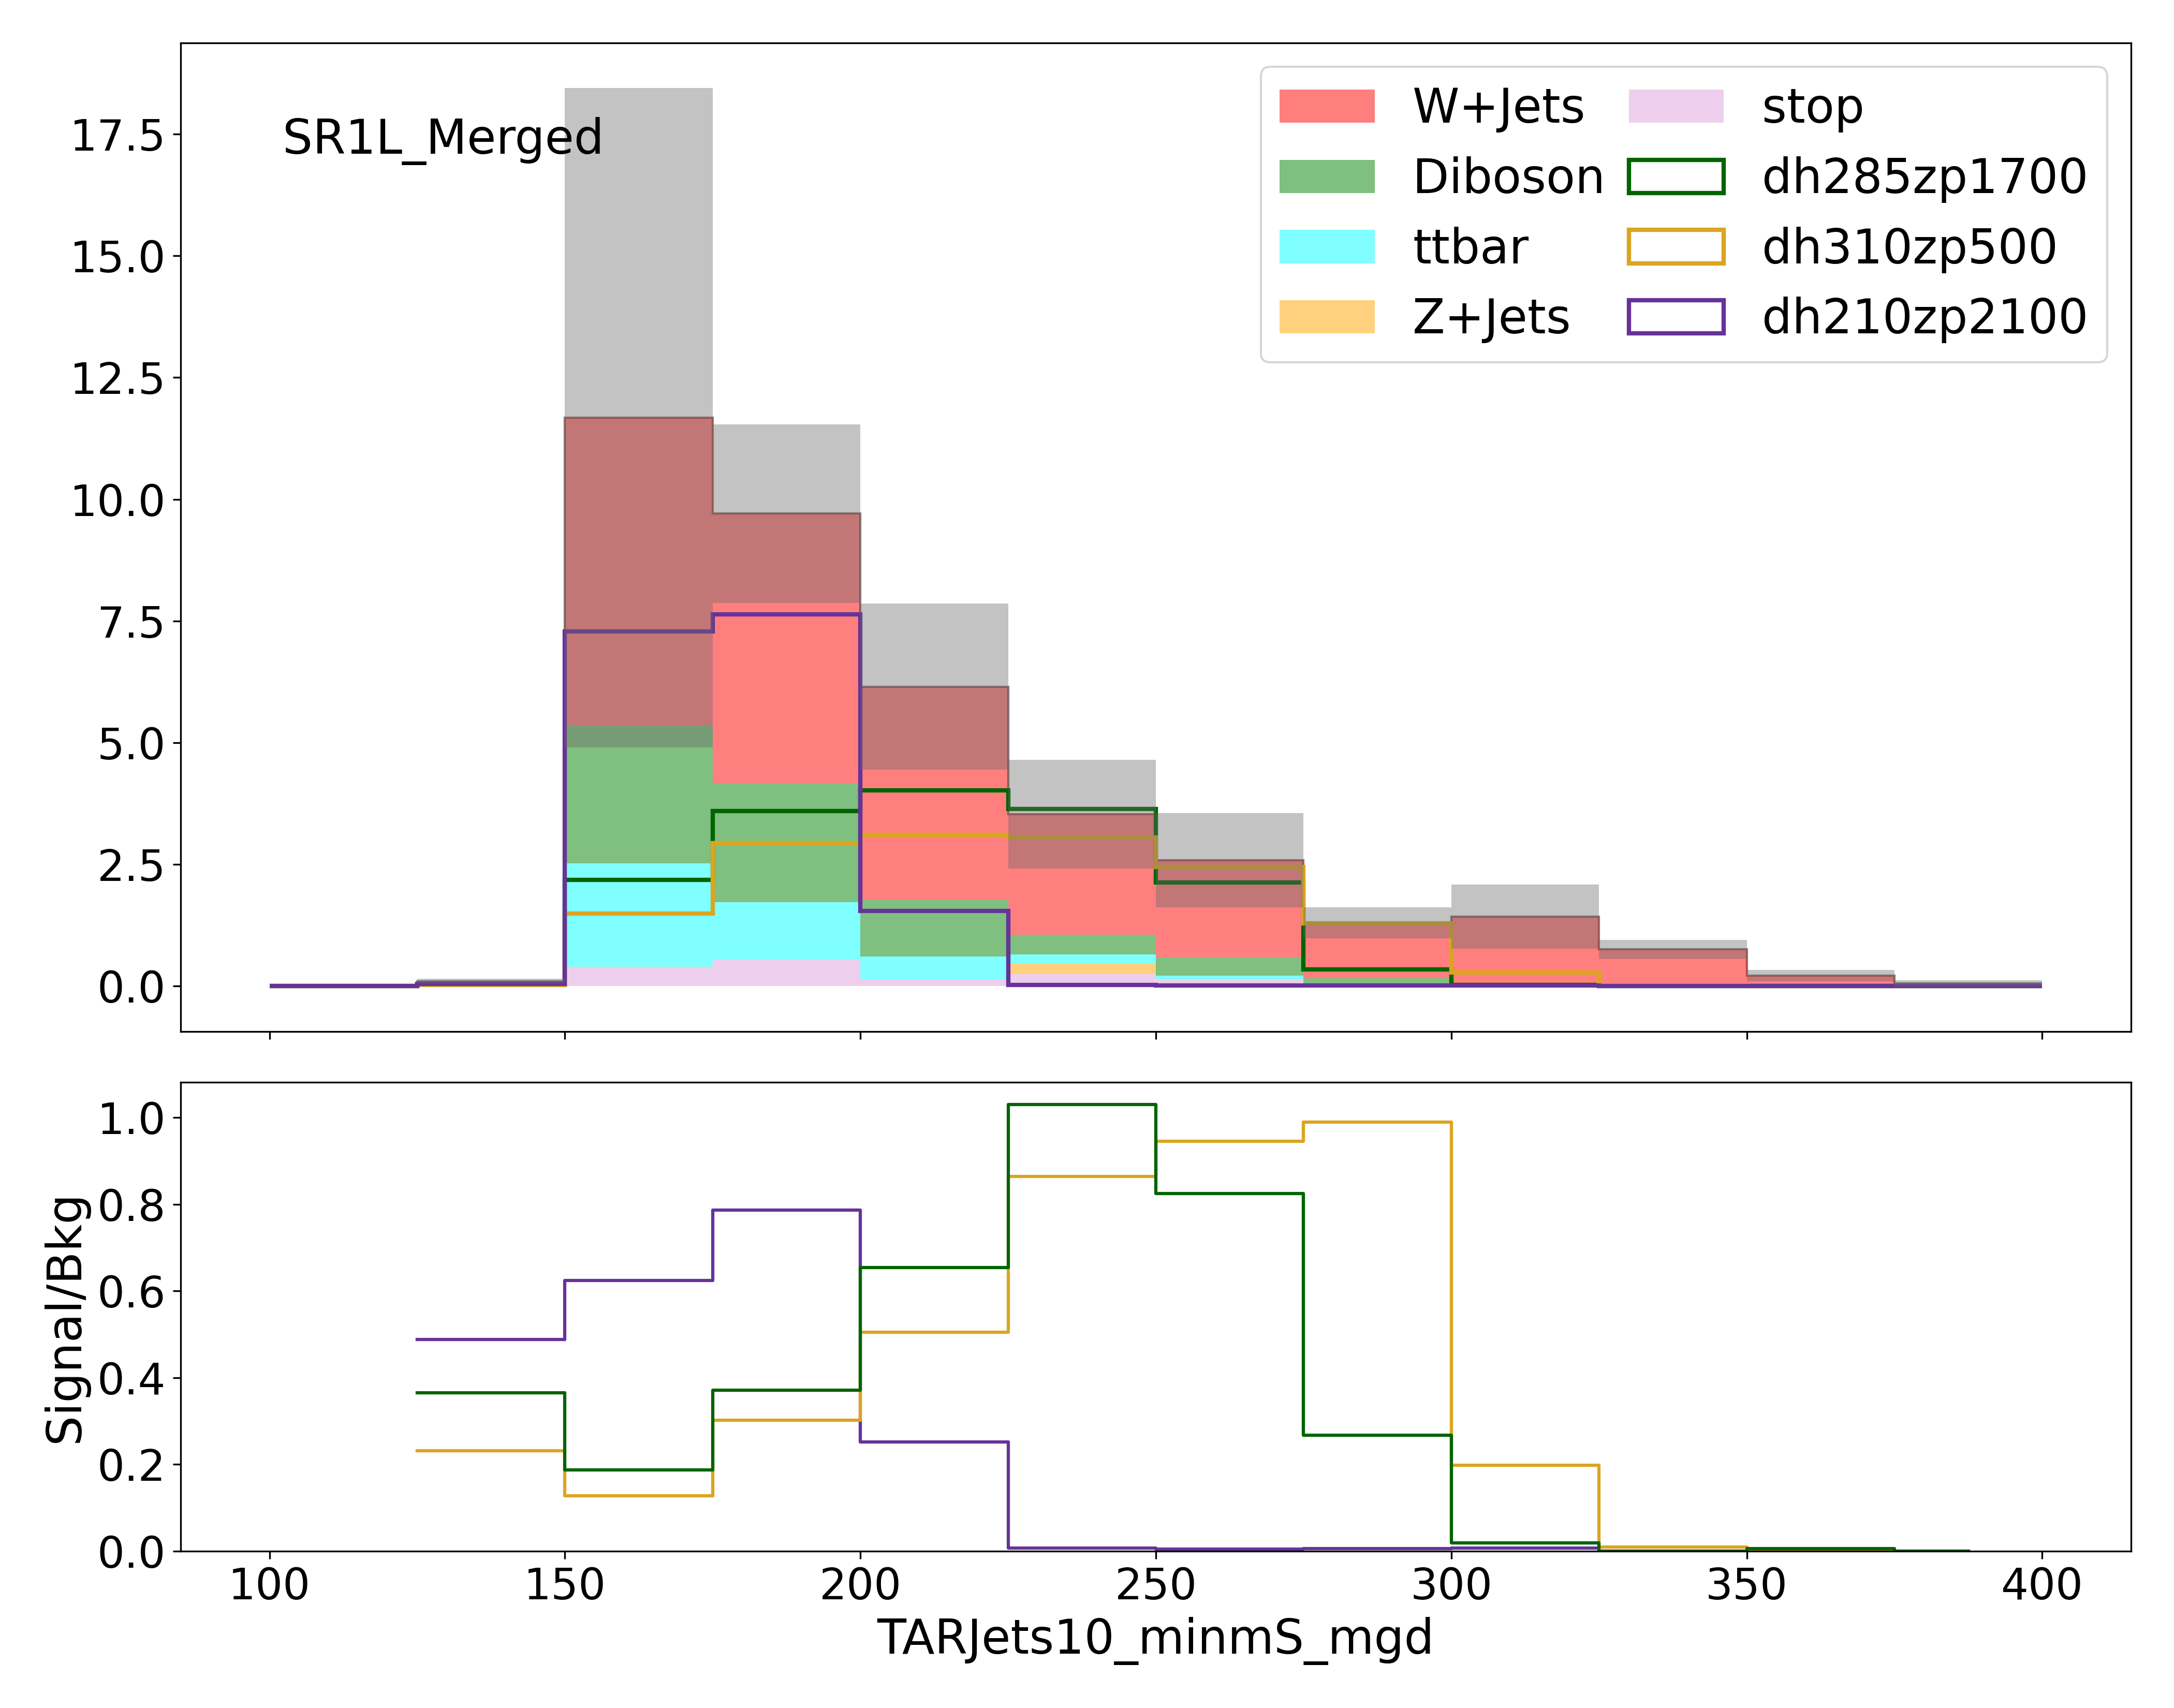
\includegraphics[width = 0.98\textwidth]{Figures/5/ms/SR1L_Merged/TARJets10_minmS_mgd.png}
     \caption{``Merged" SR}
     \end{subfigure}
     \begin{subfigure}{0.49\textwidth}
     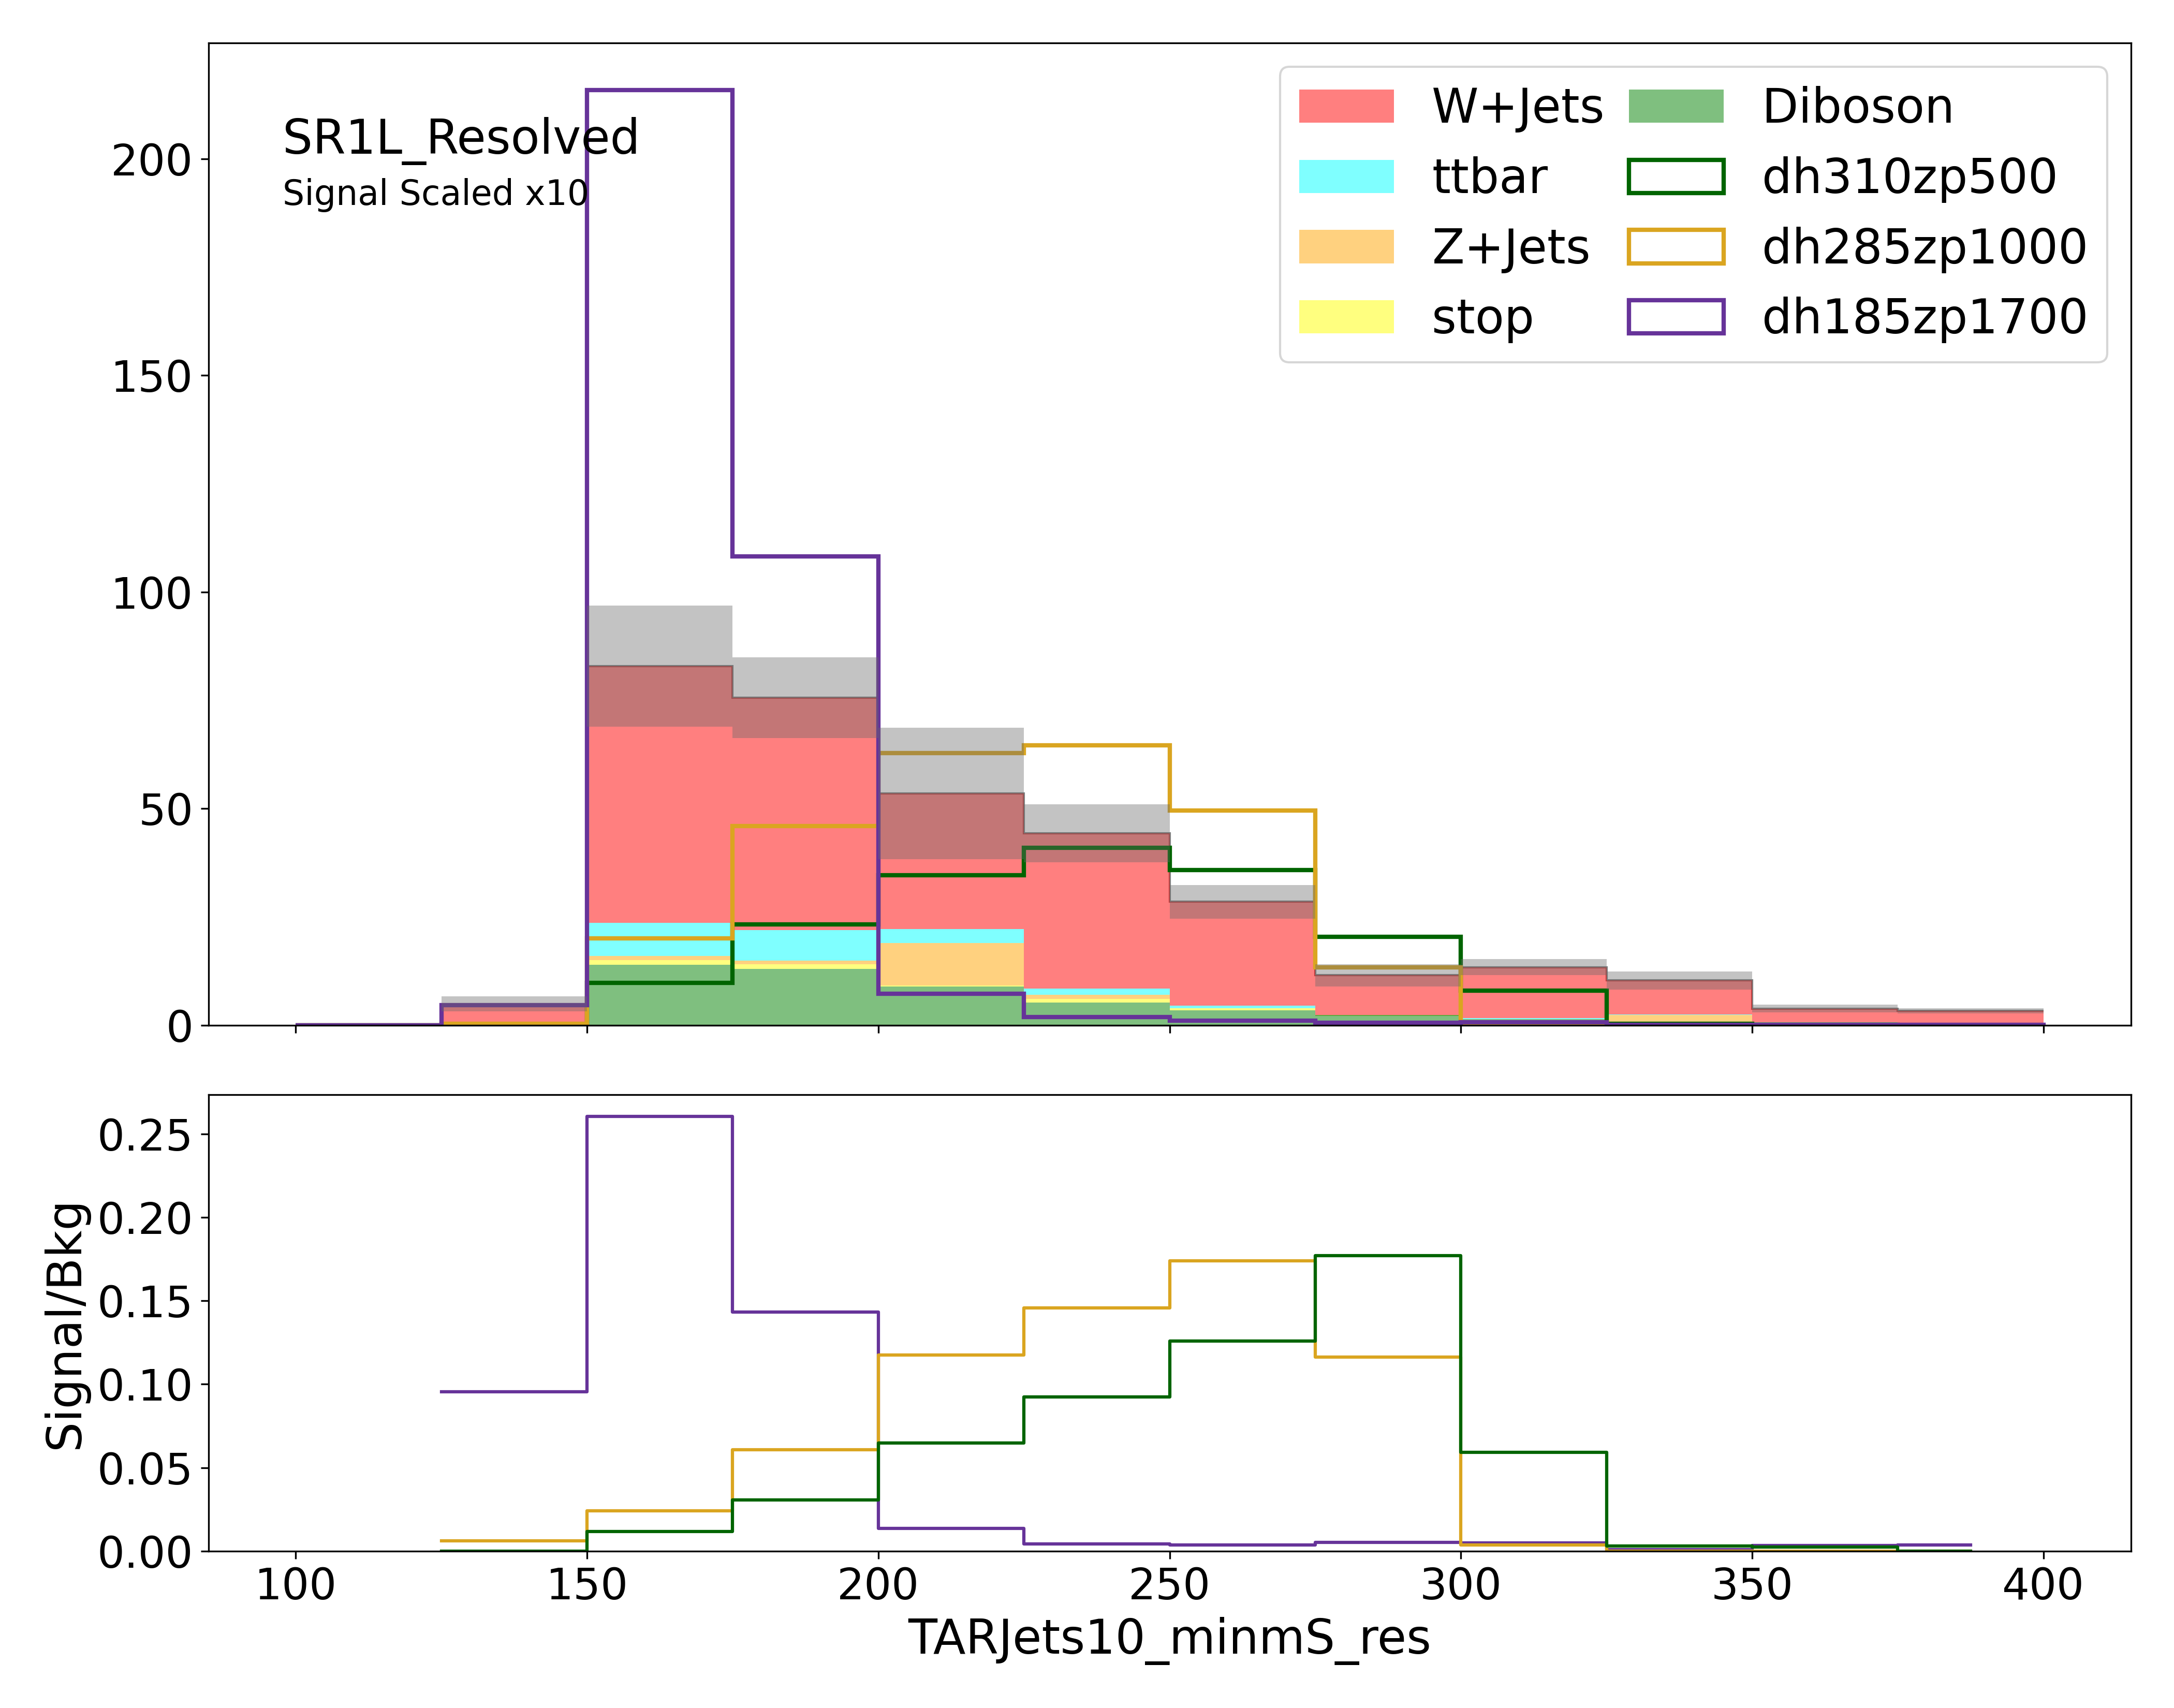
\includegraphics[width = 0.98\textwidth]{Figures/5/ms/SR1L_Resolved/TARJets10_minmS_res.png}
     \caption{``Resolved" SR}
     \end{subfigure}

     \caption{Distributions of \minms in the \merged and \resolved signal regions.}
     \label{fig:ms}
  \end{figure}

\section{Systematic Uncertainties}
While statistical fluctuations are uncorrelated between measurements and arise from a measurement consisting of a limited number of observations, systematic uncertainties are often correlated across repeated measurements, generally do not scale with the sample size, and may derive from the nature of the experiment or uncertainty in the model used to make conclusions about the data.  For this analysis we further categorize systematic uncertainties into theory uncertainties on the modelling and experimental uncertainties. The evaluation of theory uncertainties on is not within the scope of this thesis, and they are given a flat value of 20\% of the yield on each background category. A short description of the various types of experimental systematic uncertainties considered follows.

\subsection{$R=0.4$ Jets}
Uncertainties on $R=0.4$ jets are divided into jet energy scale (JES) and jet energy resolution (JER) uncertainties. These include, but are not limited to, uncertainties on pileup, flavour composition, and punch-through of jets. We evaluate them using tools provided by the ATLAS Jet/\met group.

\subsection{Track Uncertainties}
These are uncertainties on the reconstruction of tracks in the ATLAS inner detector. In this analysis they are primarily propagated into the reconstruction of TAR jets in the ``merged" signal and control regions.

\subsection{Muon and Electron}
For muons and electrons we consider uncertainties on the reconstruction efficiency, isolationa and identification, and energy or momentum scale and resolution. We evaluate these uncertainties using tools provided by the ATLAS E/Gamma and Muon combined performance groups.

\subsection{\met}
We propagate uncertainties on the afformentioned objects into the \met calculation, however we consider separate \met systematics which affect the reconstruction of the \met soft term. We evaluate these using the METSystematicsTool.

\subsection{Luminosity}
The integrated luminosity measured across the data-taking periods considered is known to a precision of 1.7\%. This is therefore applied as a an overall systematic across the normalization of all MC events.

\section{Fit Results}
\subsection{Background only fit}
I first perform a background-only fit to examine the effects of systematic uncertainties and control region normalization on background yield predictions in the signal regions.
\subsection{Exclusion contours}
